%%This is a very basic article template.
%%There is just one section and two subsections.
\documentclass{scrartcl}
\usepackage[colorlinks, urlcolor=blue]{hyperref}
\usepackage{fullpage}
\usepackage{graphics}
\usepackage{graphicx}
\usepackage{verbatim}
\usepackage{upquote}

\title{Ohmage Installation and Administration Manual for Fedora}
\subtitle{Version 2.14-0}


\begin{document}

\maketitle

\noindent Feedback, bugs, comments, suggestions, etc, about the installation
packages or this document are welcome and can go to \href{mailto:jeroen.ooms@stat.ucla.edu}{jeroen.ooms@stat.ucla.edu}.
Communication about the Ohmage software itself is easiets through github:
\href{https://github.com/cens/ohmageServer}{https://github.com/cens/ohmageServer}.

\section*{About}

\noindent The following instructions will deploy a server with \texttt{ohmage
2.14}. For this version of Ohmage, builds are available for Fedora versions 17 and 18.
The software consists of two packages:

\begin{itemize}
  \item \texttt{ohmage-server}
  \item \texttt{ohmage-selfreg} 
\end{itemize}

\noindent The \texttt{ohmage-server} package installs the server and
admin front-end. Dependencies include:

\begin{itemize}
  \item \texttt{mysql-server}
  \item \texttt{tomcat}
  \item \texttt{httpd}
  \item \texttt{mod\_ssl}
\end{itemize}

\noindent The \texttt{ohmage-selfreg} package enables \emph{self-registration}
on the ohmage server. Dependencies are:

\begin{itemize}
  \item \texttt{ohmage-server}
  \item \texttt{MTA} (mail transfer agent)
\end{itemize}

\noindent When installing a package, the package manager will automatically
install any required dependencies if not installed yet.


\section{Installation}

The current version of ohmage has builds available for Fedora 17 and 18.
If you already have a Fedora system set up, you can skip this section and
move to section \ref{preparations}.
If you do not have a local Fedora system available, you can still use
the packages by running Fedora on Amazon EC2. The easiest way to get started is
to load an instance with one of the official Fedora cloud images: \\

\url{https://fedoraproject.org/wiki/Cloud_images} \\

\noindent Another possibility is to install a Ohmage on a virtual Fedora server
inside another OS. For example, the free VMware Player is available for Windows 
and Linux, and on OSX one can use parallels to run an Fedora server. This way
you can install Fedora and Ohmage safely on top of an existing system.

\subsection{Preparations}
\label{preparations}

Before installation, make sure you are running Fedora 17 or 18, and that your
package are up to date, and that \texttt{wget} is installed:

\begin{verbatim}
    sudo yum update
    sudo yum install wget
\end{verbatim}

\noindent Also make sure that no conflicting software installed on the system.
For example, remove any copies of Tomcat or MySQL that you downloaded and
installed manually from the Oracle website (instead of using \texttt{yum}).
Those might conflict with the \texttt{mysql-server} and \texttt{tomcat}
packages that ship with fedora. Anything previously installed through
\texttt{yum} is fine.

\subsection{Adding the Ohmage Repository}

We first add the repository containing the ohmage packages to our system. On
Fedora 18:

\begin{verbatim}
  cd /etc/yum.repos.d/
  sudo wget http://download.opensuse.org/repositories/\
    home:jeroenooms:ohmage-2.14/Fedora_18/home:jeroenooms:ohmage-2.14.repo
\end{verbatim}

\noindent Instead, if you are running Fedora 17:

\begin{verbatim}
  cd /etc/yum.repos.d/
  sudo wget http://download.opensuse.org/repositories/\
    home:jeroenooms:ohmage-2.14/Fedora_17/home:jeroenooms:ohmage-2.14.repo
\end{verbatim}

\subsection{Installing the server}

After the repositories have been added, we can use \texttt{yum} to install
Ohmage. To install the Ohmage server and front-end, use:

\begin{verbatim}
   sudo yum install ohmage-server
\end{verbatim}

\noindent Select \texttt{[y]} when the package manager prompts for confirmation.
After installation has completed, you can test the installation using curl:

\begin{verbatim}
    curl --insecure https://localhost/app/config/read
\end{verbatim}

\noindent If OK, open a browser and naviage to the front-end, e.g:
\url{https://example.com/ohmage}.

\subsection{Enabling self registration}

Self registration is not required to run ohmage. To enable self registration on
the server, run the following line:
\begin{verbatim}
   sudo yum install ohmage-selfreg
\end{verbatim}
This will install an SMTP server and enable the Ohmage self-registration module.
After installing, open the administration front-end page in the browser. If the
self registration button does not show up yet, wait a minute and force a full
refresh in the browser (\texttt{CTRL+R}).

\subsection{Uninstall Ohmage}

To completely remove Ohmage from a system, run:

\begin{verbatim}
    sudo yum remove ohmage-server
\end{verbatim}
Note that this will delete all data including the \texttt{ohmage} database.

\section{Administration}

The \texttt{ohmage-server} packages installs 2 sites:

\begin{itemize}
  \item Ohmage Server: \url{http://example.com/app/config/read}
  \item Ohmage Front-end: \url{http://example.com/ohmage}
\end{itemize}

\noindent After installation, visit the administration front-end to setup the
administrator account: \url{https://example.com/ohmage}. After a new
installation, one can authenticate using the default username and password
\texttt{ohmage.admin} with \texttt{ohmage.passwd}. At first login, you will be
prompted to change this password. By default, both http and https are enabled.
However, the https is served by a self-signed a.k.a. \emph{snakeoil} SSL
certificate, so the browser will give a warning about insecure encryption.
For more info see the section \ref{ssl} of this manual.

\subsection{Tomcat in Fedora}

Fedora 17 and 18 ship with Tomat7. The Tomcat server hosts the AJP1.3 protocol
on port 8009. Actual incoming HTTP and HTTPS are handled by Apache2 and proxied
to Tomcat. To manage the Tomcat server do:

\begin{verbatim}
    sudo service tomcat {start | stop | restart}
\end{verbatim}

Tomcat configuration files, for example \texttt{server.xml} are located at

\begin{verbatim}
    /etc/tomcat/
\end{verbatim}

The tomcat log files, e.g. \texttt{catalina.out} are located in Fedora at

\begin{verbatim}
    /var/log/tomcat/
\end{verbatim}
The \texttt{webapps} directory, hosting the \texttt{.war} files is located at

\begin{verbatim}
    /var/lib/tomcat/webapps/
\end{verbatim}

\subsection{Apache2 (httpd) in Fedora}

Incoming requests on port 80 (HTTP) and port 443 (HTTPS) are handled by the
Apache2 webserver. Apache2 is also called \texttt{httpd} in fedora. The
\texttt{mod\textunderscore proxy\textunderscore ajp} module is used to proxy
requests to Tomcat server. To manage Apache2 use:

\begin{verbatim}
    sudo service httpd {start | stop | restart}
\end{verbatim}
The main configuration file for apache2 is located at

\begin{verbatim}
    /etc/httpd/conf/httpd.conf
\end{verbatim}
This file should rarely be edited. Custom configurations includes are located
at:

\begin{verbatim}
    /etc/httpd/conf.d/
\end{verbatim}
For example, the \texttt{/app} and \texttt{/ohmage} proxy sites are defined in
\begin{verbatim}
    /etc/httpd/conf.d/ohmage.conf
\end{verbatim}
The Apache2 log files \texttt{access.log} and \texttt{error.log} are located at

\begin{verbatim}
    /var/log/httpd/
\end{verbatim}

\subsection{MySQL}

The MySQL server can be managed through:

\begin{verbatim}
    sudo service mysqld {start|stop|restart}
\end{verbatim}

The mysql configuration file on Fedora is located at:

\begin{verbatim}
   /etc/my.conf
\end{verbatim}
In general, it should not be required to manually enter mysql for using Ohmage.
But if for some reason this is needed, you can connect to the mysql server
using:

\begin{verbatim}
    mysql -u'ohmage' -p'&!sickly'
\end{verbatim}
The password is \texttt{\&!sickly} and all ohmage data is stored in database
\texttt{ohmage}.

\subsection{SSL certificate}
\label{ssl}

By default, Apache2 uses self signed a.k.a. snakeoil certificates. This is
convenient for development servers, but in a production setting these
should be replaced by SSL certificates signed by an official Certificate Authority. \\

\noindent The https configurations and locations of the certificates are defined
in

\begin{verbatim}
    /etc/httpd/conf.d/ssl.conf
\end{verbatim}
This file also contains detailed comments with configuration instructions.

\subsection{Self registration}
\label{selfreg}

Ohmage supports option self registration. This means that users can register an 
account for themselves without any help from an administrator. The self
registration module can be installed as follows:

\begin{verbatim}
    sudo yum install ohmage-selfreg
\end{verbatim}

\noindent As part of the self registration process, a user will receive an email
with a confirmation code, and a link back to the server. In order for this to
work properly, the server needs a valid hostname. The hostname of the server is
defined in this file:

\begin{verbatim}
    /etc/hostname
\end{verbatim}

\noindent The link that is included in the confirmation email that self
registered user receive, is determined by this file, so make sure it contains a
proper hostname, and not e.g. \texttt{localhost} or some internal name. \\

\noindent The self registration depends on a properly functioning
SMTP server on the system, either Postfix or Sendmail. These will automatically
be installed when installing \texttt{ohmage-selfreg}. During the installation of
Postfix you might be propted for the hostname of your server. Again, make sure
that you enter a valid hostname here that can be reached through the internet.

\subsubsection{Important: Reverse DNS and Spam Detection}

Because spam is a big problem these days, most email providers tend to flag
emails that have been send from anonymous SMTP servers as spam. As a result,
the self registration confirmation emails might end up in their spam-folder or
junkmail. In order to minimize the chance that emails from Ohmage end up in spam
filters, it is highly recommended to use a domain that you actually purchased,
and not just the hostname of the machine that your ISP/hosting partner provided.
Furthermore it is important that the \emph{\textbf{reverse DNS}} of the server
to points back to this same domain name. Setting the reverse DNS is a process
that only your hosting provider can do for you. Most providers require you to
request this manually, for example, on EC2 you have to fill out this form: \\

{\footnotesize\url{https://aws-portal.amazon.com/gp/aws/html-forms-controller/contactus/ec2-email-limit-rdns-request}}
\\



\noindent In order to test if the the DNS and Reverse DNS are working properly,
you can use a command like \texttt{nslookup} on Linux or \texttt{tracert} on
Windows. Alternatively you can use a free web tool to do the lookup for you,
for example \url{http://www.dnsgoodies.com/}.

 



\subsection{Other Ohmage files}

Photos, videos and documents uploaded by users are stored in

\begin{verbatim}
    /var/lib/ohmage/images/
    /var/lib/ohmage/documents/
    /var/lib/ohmage/videos/
\end{verbatim}
Log files for ohmage can be found in:

\begin{verbatim}
    /var/log/ohmage
\end{verbatim}

\noindent Note that these are only high level ohmage logs. If there are problems
with the web server or database itself, these might appear in the tomcat logs. 
Finally, some static files included in the installation packages (scripts,
war files) can be found at:

\begin{verbatim}
    /usr/lib/ohmage/
\end{verbatim}

\section{Clients}

Currently there are 3 clients for the Ohmage server system. These are:

\begin{itemize}
  \item The Ohmage Android App.
  \item The Ohmage FrontEnd.
  \item The Ohmage R package.
\end{itemize}
Below a brief description of these clients.

\subsection{The Ohmage Android App}

The Ohmage Android 'app' is the application on the mobile phone that can be used
to fill out surveys and upload survey-responses to the server. As it currently
stands, the server-url is hardcoded in the app and therefore the app has to be
built from source. Figure \ref{fig:phone} shows a screenshot of the phone app running on
an Android 2.2 device. \\

\begin{figure}[h!]
\begin{center}
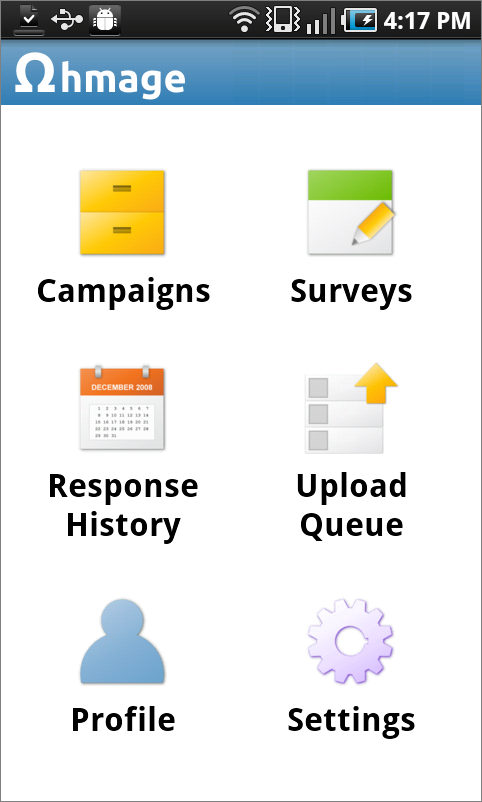
\includegraphics[width=4cm]{app.png}
\caption{A screenshot of the Android app.}
\label{fig:phone}
\end{center}
\end{figure}

\noindent The Android app can be downloaded from Google Play on any
Android phone by searching for \texttt{ohmage}. More information about the
app is available at: \\

\url{https://play.google.com/store/apps/details?id=org.ohmage} \\

When running the app for the first time after installing it from Google play, it
will prompt the user for the server address of the Ohmage server.
Alternatively, the app can be build from source. This way, the app can be
distributed with a hardcoded server address. The source code and instructions on
how to build the app are publicly available on: \\

\url{https://github.com/cens/ohmagePhone} \\

\subsection{The Ohmage FrontEnd}

The Ohmage FrontEnd is an administrative web application to be used on a regular
browser by both users and administrators of Ohmage. The application is
automatically installed when installing the server using instructions above and
available through: \url{http://example.com/ohmage}. Source code and
development of the FrontEnd is publicly available on github at
\url{https://github.com/cens/ohmageFrontEnd}. Figure \ref{fig:frontend} shows a
screenshot of the FrontEnd homepage after logging in. \\

\noindent The FrontEnd is a convenient client to review, share and explore data,
add/remove users, classes, campaigns, perform administrative tasks, etc. The
frontend can be build with some custom skinning options. The screenshot shows a build of
Ohmage with the default theme.

\begin{figure}[h!]
\begin{center}
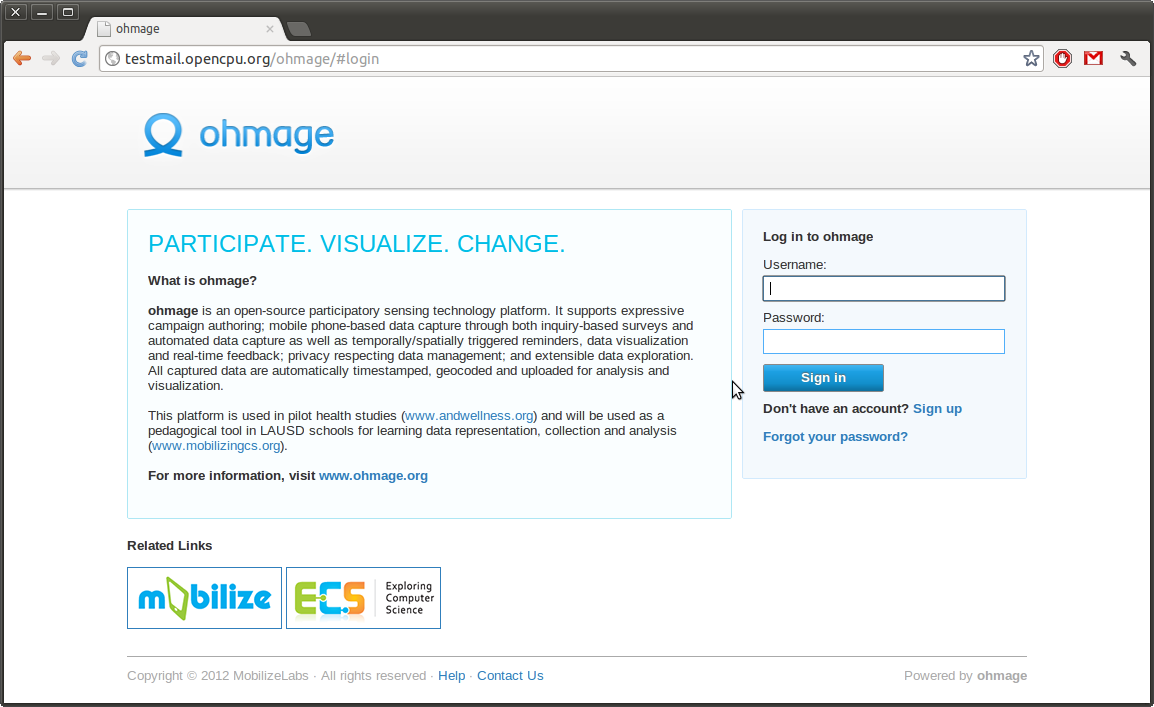
\includegraphics[width=15cm]{frontend.png}
\caption{A screenshot of the FrontEnd homepage.}
\label{fig:frontend}
\end{center}
\end{figure}

\subsection{The Ohmage \texttt{R} package}

The Ohmage R package is an Ohmage client for R. It depends on other R packages
like RCurl, XML and RJSONIO to do it's work. The package is mostly a convenient
way to grab data from Ohmage and turn it into a data frame in R. Package and
documentation are available from CRAN:
\url{http://cran.r-project.org/web/packages/Ohmage}. Below a code snippet to
illustrate the functionality of the package.

\begin{verbatim}
  library(Ohmage);
  oh.login("ohmage.admin", "mypassword", "https://myserver.com/app");
  campaigns <- oh.campaign.read();
  mydata <- oh.survey_response.read("urn:campaign:myschool:food");
\end{verbatim}

\section{Getting Started}

To understand how to use the Ohmage system, it is important to get familiar with
the basic concepts and terminology.  

\subsection{Survey terminology}

The Ohmage system is used for deploying surveys on mobile phones. These surveys
are defined in \emph{campaigns} using \texttt{XML} files. A user with
appropriate privileges can then upload such an XML file to the Ohmage server in
order to deploy the survey. Some essential concepts:

\begin{itemize}
  \item A \texttt{campaign} is an \texttt{XML} file which describes one or more
  \texttt{surveys}. 
  \item A \texttt{survey} is a set of survey questions called \texttt{prompts}.
  \item A \texttt{prompt} is a single question inside a survey. There are
  several \texttt{prompt types}. The prompt type specifies how the question is
  displayed in the phone, and how it is stored on the server.
\end{itemize}

\noindent A basic outline of the XML structure of a campaign is outlined below.

\begin{verbatim}
    <campaign>
      ... 
      <surveys>
        <survey>
          <id>snack</id>
          <title>snack survey</title>
          ...
          <prompt> ... </prompt>
          <prompt> ... </prompt>
          <prompt> ... </prompt>
        </survey>
        <survey>
          ...
        </survey>
      </surveys>
    </campaign>
\end{verbatim}

\noindent More details and examples on how to write a campaign can be found on
the wiki page:
\url{https://github.com/cens/ohmageServer/wiki/Campaign-Definition}.

\subsection{Users, Roles and Classes}
Users, roles and classes are the central concepts that control access to Ohmage.
A user is a person who can authenticate with the system and perform certain
actions. Users can either be created by an administrator, or self created,
when self registration is enabled on the server.\\

Users are organized in groups called \texttt{classes}. To give users access to a
campaign, the users has to be added to a class that is associated with this
campaign.\\

Permissions of users are defined using \texttt{roles}. There are two types of
roles: \texttt{class roles} and \texttt{campaign roles}. A user can have the
class role of \texttt{admin}, \texttt{privileged} or \texttt{restricted}. 
For each campaigns, the user can have any of the following roles:
\texttt{participant}, \texttt{analyst}, \texttt{author}, or \texttt{supervisor}.
For detailed descriptions on how classes and roles are used to manage user
access, consult this wiki page:\\

\url{https://github.com/cens/ohmageServer/wiki/About-Users,-Classes-and-Campaigns}



\subsection{Prompt types}

The prompt type is another central concept in the Ohmage system. Inside the XML
file, each survey lists one or more \texttt{prompts}. These prompts represent
survey questions. Each prompt has a \texttt{promptType} attribute, which defines
what kind of question this is. The promptType determines how the question is
displayed on the phone, how it is saved on the server, and what it looks like
when data is exported from the server. \\

Each prompt type has its own unique properties. These properties are used to
configure the question. The most important prompt types include:

\begin{itemize}
  \item \texttt{number} -- Displays a number field. Properties include
  \texttt{min} and \texttt{max}.
  \item \texttt{single\_choise} -- Displays a ``multiple choice'' radiobutton
  question with only one answer. Properties include a list of possible answers.
  \item \texttt{multi\_choice} -- Displays a ``multiple choice'' checkbox
  question where more than one answer can be checked. Properties include a list of
  possible ansers.
  \item \texttt{text} -- Displays a free text field.
  \item \texttt{photo} -- Allows the user to take a picture.
\end{itemize}

\noindent A more extensive list of different prompt types and their properties
is available here: \\

\url{https://github.com/cens/ohmageServer/wiki/Campaign-Definition#wiki-promptTypes}

\subsection{Work flow}

Below the steps that outline the work flow of using Ohmage. We assume the ohmage
server and front-end are installed using the \texttt{ohmage-server} package as
described in section 2.\\

\noindent The researcher first has to create a campaign and deploy it to the
users. These steps include:

\begin{enumerate}
  \item Write a campaign XML file that defines the survey questions.
  \item Deploy the XML on the server (using admin front-end)
  \item Create a class and associate it with the campaign (using admin
  front-end)
  \item Create ohmage user accounts for all participants and add them to
  the class.
  \item Notify your participants of the server address, and their
  username/password.
\end{enumerate}

\noindent Next, the participants can fill out the surveys

\begin{enumerate}
  \item Install the \texttt{ohmage} app on their phone.
  \item Login to the ohmage server with their username and password.
  \item Enroll in one of the campaigns they have access to.
  \item Fill out any survey as many times as desired.
\end{enumerate}

\noindent Finally, at any time the researcher can view and export responses from
the server. The administration front-end has some basic tools of exporting data
in e.g. CSV format.

\end{document}
